\section{Systemarchitektur und Methodik}
\label{sec:systemarchitektur_und_methodik}

Die methodische Umsetzung erfolgt über eine Pipeline, die in der Programmiersprache Python implementiert ist.
Hierbei kommen Frameworks wie \texttt{Scikit-learn} für die Machine-Learning-Verfahren und \texttt{PyTorch} zum Einsatz.
Das Gesamtsystem ist darauf ausgelegt, die Anforderungen an Robustheit, Integration äußerer Faktoren, probabilistische Prognosen und Transparenz zu erfüllen.

\begin{figure}[hpt!]
\centering
	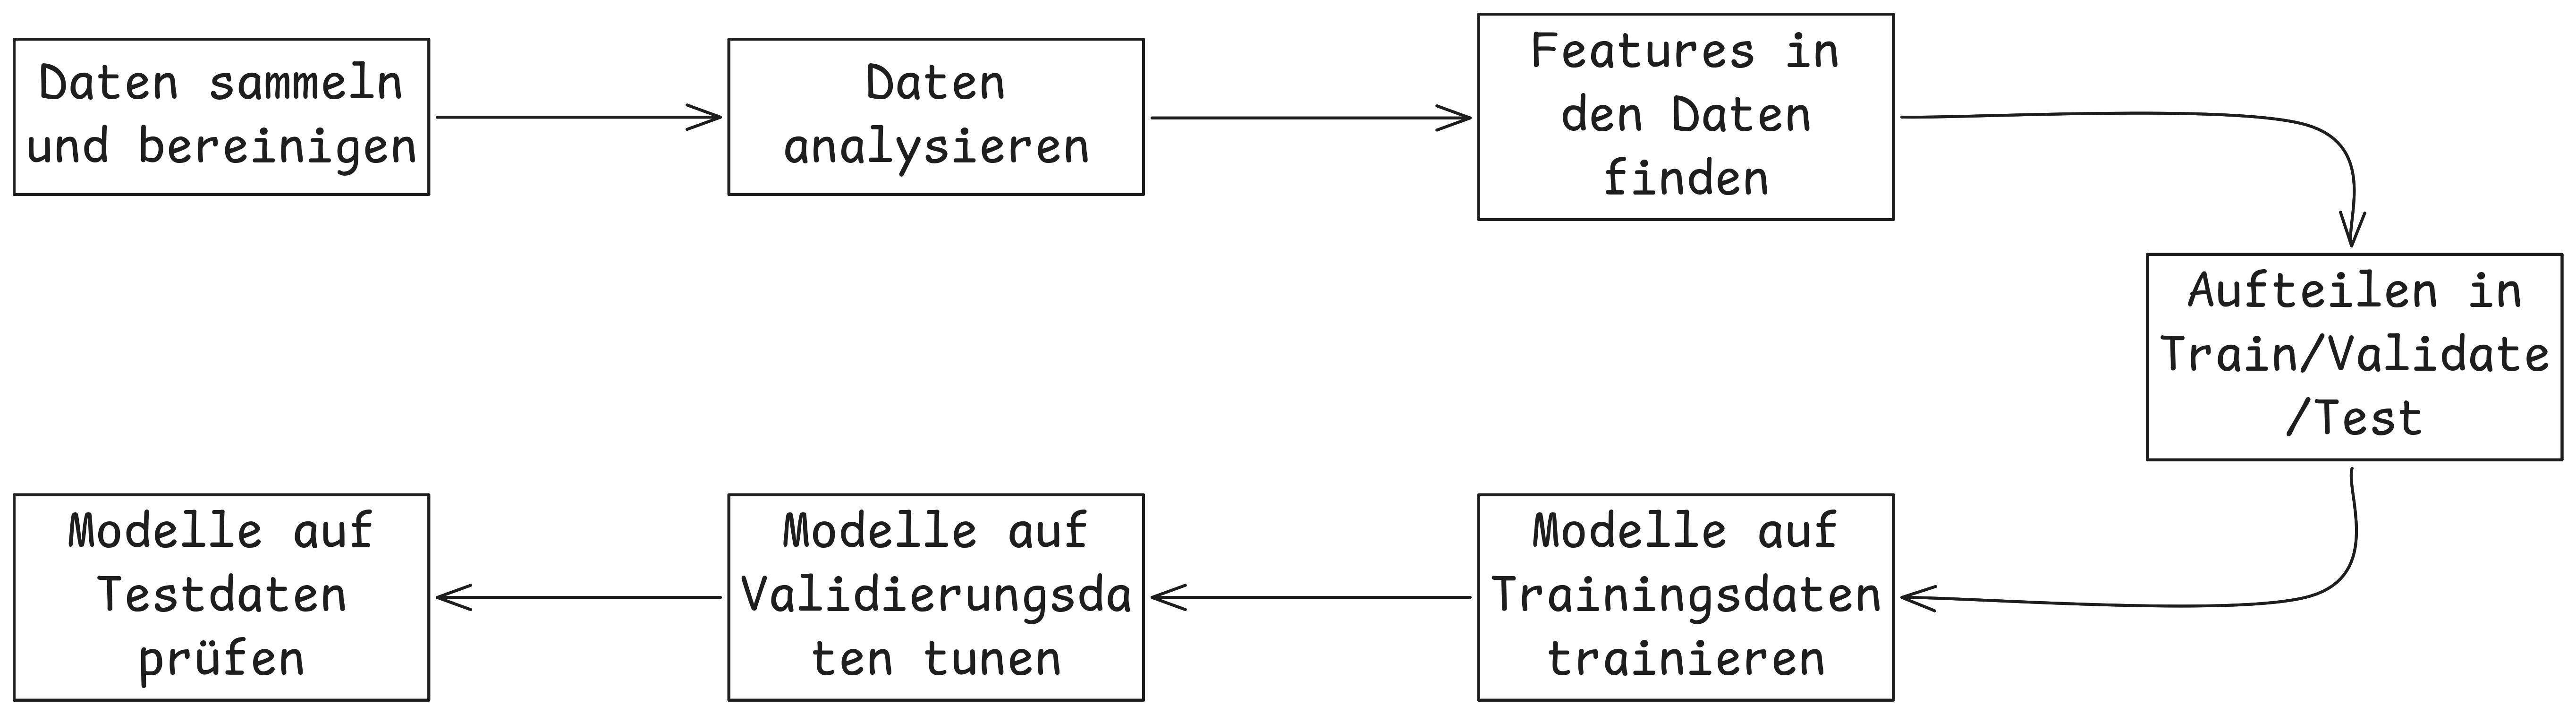
\includegraphics[width=0.9\linewidth]{./img/model_pipeline.png}
	\caption{Grobe Schematische Darstellung der Systemarchitektur: Von der Datenvorverarbeitung über die Merkmalsextraktion bis zur Walk-Forward-Validierung.}
    \label{fig:pipeline}
\end{figure}

\subsection{Feature Engineering}
Um dem Modell Kontext über die zeitliche Dynamik und Marktinterdependenzen zu geben, werden über 1.
00 Merkmale (Features) generiert. Diese lassen sich in Gruppen unterteilen:

\subsubsection{Lag-Features}
Hierbei werden die Preis- und Volumenwerte der vorangegangenen 14 Tage beispielsweise als zusätzliche Eingabedimensionen genutzt.
Dies erlaubt es dem Modell, kurzfristige Autokorrelationen in der Zeitreihe zu identifizieren.

\subsubsection{Rolling Windows}
Es werden statistische Kennzahlen (Mittelwert, Standardabweichung, Minimum, Maximum) über gleitende Zeitfenster von 3, 6 und 12 Tagen beispielsweise berechnet.
Diese dienen als Glättungsfilter und erlauben die Erkennung von Trends und Volatilitätsänderungen.

\subsubsection{Volatilitäts-Features (GARCH-Proxy)} 
Mittels exponentiell gewichteter gleitender Durchschnitte wird die Volatilität für Zeitspannen von beispielsweise 5, 10 und 21 Tagen geschätzt.
Das funktioniert, indem die jüngsten Preisänderungen stärker gewichtet werden als ältere, was eine zeitnahe Reaktion auf Marktveränderungen ermöglicht.

\subsubsection{Cross-Metal-Korrelationen} 
Rollende Pearson-Korrelationen zwischen Aluminium und den anderen Metallen (Kupfer, Gold etc.
über Fenster von 20 und 60 Tagen erfassen gegenseitig abhängige Marktbewegungen und Kapitalflüsse innerhalb des Rohstoffsektors.
Das wird durch die Berechnung der Korrelation zwischen den Log-Returns von Aluminium und den anderen Metallen über die definierten Zeitfenster erreicht.

\subsection{Regime Detection mittels KMeans}
Marktphasen unterliegen oft strukturellen Veränderungen (Regimewechsel).
Zur automatisierten Identifikation dieser Zustände kommt ein \emph{KMeans-Clustering} zum Einsatz.
Hierbei werden Datenpunkte basierend auf ihrer Ähnlichkeit in den Dimensionen Volatilität, Trend und Schiefe gruppiert.
Es werden drei Regime definiert, die unterschiedliche Marktzustände (stabil, trendfolgend, volatil) repräsentieren.
Diese Information wird als zusätzliches Merkmal in die Vorhersagemodelle integriert.

\subsection{Merkmalsauswahl (Feature Selection) mittels ExtraTrees}
Angesichts der hohen Dimensionalität des Merkmalsraums besteht die Gefahr der Überanpassung.
Zur Reduktion der Komplexität wird ein \texttt{ExtraTreesRegressor} (Extremely Randomized Trees) eingesetzt.
Dieser schätzt die Bedeutung jedes Merkmals für die Vorhersage des Zielwerts (Aluminiumpreis) und ermöglicht so eine gezielte Auswahl der relevantesten Features.
Nur Merkmale, deren Bedeutung über dem Durchschnitt liegt, werden beibehalten.
Dieser Prozess reduziert den Satz auf relevante Variablen.

\subsection{Skalierung und Vermeidung von Data Leakage}
Ein kritischer Aspekt bei der Zeitreihenprognose ist die Vermeidung von \emph{Data Leakage}, also dem ungewollten Einfließen von Informationen aus der Zukunft in den Trainingsprozess.

\subsubsection{Z-Score Standardisierung}
Um den Lernprozess der neuronalen Netze zu optimieren, werden alle Features auf einen Mittelwert von 0 und eine Standardabweichung von 1 skaliert.

\subsubsection{Lokale Skalierung}
Die Parameter für diese Skalierung werden für jeden Walk-Forward-Fold individuell und ausschließlich auf Basis der jeweiligen Trainingsdaten berechnet.
Dadurch wird sichergestellt, dass das Modell keine Kenntnis über die Varianz oder den Mittelwert der zukünftigen Validierungs- oder Testdaten besitzt.

\subsection{Validierungsstrategie: Walk-Forward Validation}
Bei Zeitreihen führt eine klassische k-fache Kreuzvalidierung zu Datenlecks (Data Leakage), da Informationen aus der Zukunft für die Vorhersage der Vergangenheit genutzt würden.
Stattdessen wird eine \emph{Walk-Forward-Validierung} implementiert.
Hierbei wird das Trainingsfenster allmählich erweitert und das Modell in jedem Schritt auf einem direkt folgenden, zeitlich begrenzten Validierungsfenster (beispielsweise 63 Tage, entspricht ca. einem Quartal) evaluiert.
Dieser Prozess wird über 32 Iterationen (\emph{Folds}) wiederholt, um eine robuste Schätzung der Modellleistung zu erhalten.
Die Ergebnisse werden summiert, um die Generalisierungsfähigkeit des Modells auf ungesehenen Daten zu simulieren.

